
%% bare_jrnl.tex
%% V1.4b
%% 2015/08/26
%% by Michael Shell
%% see http://www.michaelshell.org/
%% for current contact information.
%%
%% This is a skeleton file demonstrating the use of IEEEtran.cls
%% (requires IEEEtran.cls version 1.8b or later) with an IEEE
%% journal paper.
%%
%% Support sites:
%% http://www.michaelshell.org/tex/ieeetran/
%% http://www.ctan.org/pkg/ieeetran
%% and
%% http://www.ieee.org/

%%*************************************************************************
%% Legal Notice:
%% This code is offered as-is without any warranty either expressed or
%% implied; without even the implied warranty of MERCHANTABILITY or
%% FITNESS FOR A PARTICULAR PURPOSE! 
%% User assumes all risk.
%% In no event shall the IEEE or any contributor to this code be liable for
%% any damages or losses, including, but not limited to, incidental,
%% consequential, or any other damages, resulting from the use or misuse
%% of any information contained here.
%%
%% All comments are the opinions of their respective authors and are not
%% necessarily endorsed by the IEEE.
%%
%% This work is distributed under the LaTeX Project Public License (LPPL)
%% ( http://www.latex-project.org/ ) version 1.3, and may be freely used,
%% distributed and modified. A copy of the LPPL, version 1.3, is included
%% in the base LaTeX documentation of all distributions of LaTeX released
%% 2003/12/01 or later.
%% Retain all contribution notices and credits.
%% ** Modified files should be clearly indicated as such, including  **
%% ** renaming them and changing author support contact information. **
%%*************************************************************************


% *** Authors should verify (and, if needed, correct) their LaTeX system  ***
% *** with the testflow diagnostic prior to trusting their LaTeX platform ***
% *** with production work. The IEEE's font choices and paper sizes can   ***
% *** trigger bugs that do not appear when using other class files.       ***                          ***
% The testflow support page is at:
% http://www.michaelshell.org/tex/testflow/



\documentclass[journal]{IEEEtran}
%
% If IEEEtran.cls has not been installed into the LaTeX system files,
% manually specify the path to it like:
% \documentclass[journal]{../sty/IEEEtran}





% Some very useful LaTeX packages include:
% (uncomment the ones you want to load)


% *** MISC UTILITY PACKAGES ***
%
%\usepackage{ifpdf}
% Heiko Oberdiek's ifpdf.sty is very useful if you need conditional
% compilation based on whether the output is pdf or dvi.
% usage:
% \ifpdf
%   % pdf code
% \else
%   % dvi code
% \fi
% The latest version of ifpdf.sty can be obtained from:
% http://www.ctan.org/pkg/ifpdf
% Also, note that IEEEtran.cls V1.7 and later provides a builtin
% \ifCLASSINFOpdf conditional that works the same way.
% When switching from latex to pdflatex and vice-versa, the compiler may
% have to be run twice to clear warning/error messages.






% *** CITATION PACKAGES ***
%
%\usepackage{cite}
% cite.sty was written by Donald Arseneau
% V1.6 and later of IEEEtran pre-defines the format of the cite.sty package
% \cite{} output to follow that of the IEEE. Loading the cite package will
% result in citation numbers being automatically sorted and properly
% "compressed/ranged". e.g., [1], [9], [2], [7], [5], [6] without using
% cite.sty will become [1], [2], [5]--[7], [9] using cite.sty. cite.sty's
% \cite will automatically add leading space, if needed. Use cite.sty's
% noadjust option (cite.sty V3.8 and later) if you want to turn this off
% such as if a citation ever needs to be enclosed in parenthesis.
% cite.sty is already installed on most LaTeX systems. Be sure and use
% version 5.0 (2009-03-20) and later if using hyperref.sty.
% The latest version can be obtained at:
% http://www.ctan.org/pkg/cite
% The documentation is contained in the cite.sty file itself.






% *** GRAPHICS RELATED PACKAGES ***
%
\ifCLASSINFOpdf
\usepackage[pdftex]{graphicx}
% declare the path(s) where your graphic files are
% \graphicspath{{../pdf/}{../jpeg/}}
% and their extensions so you won't have to specify these with
% every instance of \includegraphics
% \DeclareGraphicsExtensions{.pdf,.jpeg,.png}
\else
% or other class option (dvipsone, dvipdf, if not using dvips). graphicx
% will default to the driver specified in the system graphics.cfg if no
% driver is specified.
% \usepackage[dvips]{graphicx}
% declare the path(s) where your graphic files are
% \graphicspath{{../eps/}}
% and their extensions so you won't have to specify these with
% every instance of \includegraphics
% \DeclareGraphicsExtensions{.eps}
\fi
% graphicx was written by David Carlisle and Sebastian Rahtz. It is
% required if you want graphics, photos, etc. graphicx.sty is already
% installed on most LaTeX systems. The latest version and documentation
% can be obtained at: 
% http://www.ctan.org/pkg/graphicx
% Another good source of documentation is "Using Imported Graphics in
% LaTeX2e" by Keith Reckdahl which can be found at:
% http://www.ctan.org/pkg/epslatex
%
% latex, and pdflatex in dvi mode, support graphics in encapsulated
% postscript (.eps) format. pdflatex in pdf mode supports graphics
% in .pdf, .jpeg, .png and .mps (metapost) formats. Users should ensure
% that all non-photo figures use a vector format (.eps, .pdf, .mps) and
% not a bitmapped formats (.jpeg, .png). The IEEE frowns on bitmapped formats
% which can result in "jaggedy"/blurry rendering of lines and letters as
% well as large increases in file sizes.
%
% You can find documentation about the pdfTeX application at:
% http://www.tug.org/applications/pdftex





% *** MATH PACKAGES ***
%
\usepackage{amsmath}
% A popular package from the American Mathematical Society that provides
% many useful and powerful commands for dealing with mathematics.
%
% Note that the amsmath package sets \interdisplaylinepenalty to 10000
% thus preventing page breaks from occurring within multiline equations. Use:
%\interdisplaylinepenalty=2500
% after loading amsmath to restore such page breaks as IEEEtran.cls normally
% does. amsmath.sty is already installed on most LaTeX systems. The latest
% version and documentation can be obtained at:
% http://www.ctan.org/pkg/amsmath





% *** SPECIALIZED LIST PACKAGES ***
%
%\usepackage{algorithmic}
% algorithmic.sty was written by Peter Williams and Rogerio Brito.
% This package provides an algorithmic environment fo describing algorithms.
% You can use the algorithmic environment in-text or within a figure
% environment to provide for a floating algorithm. Do NOT use the algorithm
% floating environment provided by algorithm.sty (by the same authors) or
% algorithm2e.sty (by Christophe Fiorio) as the IEEE does not use dedicated
% algorithm float types and packages that provide these will not provide
% correct IEEE style captions. The latest version and documentation of
% algorithmic.sty can be obtained at:
% http://www.ctan.org/pkg/algorithms
% Also of interest may be the (relatively newer and more customizable)
% algorithmicx.sty package by Szasz Janos:
% http://www.ctan.org/pkg/algorithmicx




% *** ALIGNMENT PACKAGES ***
%
%\usepackage{array}
% Frank Mittelbach's and David Carlisle's array.sty patches and improves
% the standard LaTeX2e array and tabular environments to provide better
% appearance and additional user controls. As the default LaTeX2e table
% generation code is lacking to the point of almost being broken with
% respect to the quality of the end results, all users are strongly
% advised to use an enhanced (at the very least that provided by array.sty)
% set of table tools. array.sty is already installed on most systems. The
% latest version and documentation can be obtained at:
% http://www.ctan.org/pkg/array


% IEEEtran contains the IEEEeqnarray family of commands that can be used to
% generate multiline equations as well as matrices, tables, etc., of high
% quality.




% *** SUBFIGURE PACKAGES ***
%\ifCLASSOPTIONcompsoc
%  \usepackage[caption=false,font=normalsize,labelfont=sf,textfont=sf]{subfig}
%\else
%  \usepackage[caption=false,font=footnotesize]{subfig}
%\fi
% subfig.sty, written by Steven Douglas Cochran, is the modern replacement
% for subfigure.sty, the latter of which is no longer maintained and is
% incompatible with some LaTeX packages including fixltx2e. However,
% subfig.sty requires and automatically loads Axel Sommerfeldt's caption.sty
% which will override IEEEtran.cls' handling of captions and this will result
% in non-IEEE style figure/table captions. To prevent this problem, be sure
% and invoke subfig.sty's "caption=false" package option (available since
% subfig.sty version 1.3, 2005/06/28) as this is will preserve IEEEtran.cls
% handling of captions.
% Note that the Computer Society format requires a larger sans serif font
% than the serif footnote size font used in traditional IEEE formatting
% and thus the need to invoke different subfig.sty package options depending
% on whether compsoc mode has been enabled.
%
% The latest version and documentation of subfig.sty can be obtained at:
% http://www.ctan.org/pkg/subfig




% *** FLOAT PACKAGES ***
%
%\usepackage{fixltx2e}
% fixltx2e, the successor to the earlier fix2col.sty, was written by
% Frank Mittelbach and David Carlisle. This package corrects a few problems
% in the LaTeX2e kernel, the most notable of which is that in current
% LaTeX2e releases, the ordering of single and double column floats is not
% guaranteed to be preserved. Thus, an unpatched LaTeX2e can allow a
% single column figure to be placed prior to an earlier double column
% figure.
% Be aware that LaTeX2e kernels dated 2015 and later have fixltx2e.sty's
% corrections already built into the system in which case a warning will
% be issued if an attempt is made to load fixltx2e.sty as it is no longer
% needed.
% The latest version and documentation can be found at:
% http://www.ctan.org/pkg/fixltx2e


%\usepackage{stfloats}
% stfloats.sty was written by Sigitas Tolusis. This package gives LaTeX2e
% the ability to do double column floats at the bottom of the page as well
% as the top. (e.g., "\begin{figure*}[!b]" is not normally possible in
% LaTeX2e). It also provides a command:
%\fnbelowfloat
% to enable the placement of footnotes below bottom floats (the standard
% LaTeX2e kernel puts them above bottom floats). This is an invasive package
% which rewrites many portions of the LaTeX2e float routines. It may not work
% with other packages that modify the LaTeX2e float routines. The latest
% version and documentation can be obtained at:
% http://www.ctan.org/pkg/stfloats
% Do not use the stfloats baselinefloat ability as the IEEE does not allow
% \baselineskip to stretch. Authors submitting work to the IEEE should note
% that the IEEE rarely uses double column equations and that authors should try
% to avoid such use. Do not be tempted to use the cuted.sty or midfloat.sty
% packages (also by Sigitas Tolusis) as the IEEE does not format its papers in
% such ways.
% Do not attempt to use stfloats with fixltx2e as they are incompatible.
% Instead, use Morten Hogholm'a dblfloatfix which combines the features
% of both fixltx2e and stfloats:
%
% \usepackage{dblfloatfix}
% The latest version can be found at:
% http://www.ctan.org/pkg/dblfloatfix




%\ifCLASSOPTIONcaptionsoff
%  \usepackage[nomarkers]{endfloat}
% \let\MYoriglatexcaption\caption
% \renewcommand{\caption}[2][\relax]{\MYoriglatexcaption[#2]{#2}}
%\fi
% endfloat.sty was written by James Darrell McCauley, Jeff Goldberg and 
% Axel Sommerfeldt. This package may be useful when used in conjunction with 
% IEEEtran.cls'  captionsoff option. Some IEEE journals/societies require that
% submissions have lists of figures/tables at the end of the paper and that
% figures/tables without any captions are placed on a page by themselves at
% the end of the document. If needed, the draftcls IEEEtran class option or
% \CLASSINPUTbaselinestretch interface can be used to increase the line
% spacing as well. Be sure and use the nomarkers option of endfloat to
% prevent endfloat from "marking" where the figures would have been placed
% in the text. The two hack lines of code above are a slight modification of
% that suggested by in the endfloat docs (section 8.4.1) to ensure that
% the full captions always appear in the list of figures/tables - even if
% the user used the short optional argument of \caption[]{}.
% IEEE papers do not typically make use of \caption[]'s optional argument,
% so this should not be an issue. A similar trick can be used to disable
% captions of packages such as subfig.sty that lack options to turn off
% the subcaptions:
% For subfig.sty:
% \let\MYorigsubfloat\subfloat
% \renewcommand{\subfloat}[2][\relax]{\MYorigsubfloat[]{#2}}
% However, the above trick will not work if both optional arguments of
% the \subfloat command are used. Furthermore, there needs to be a
% description of each subfigure *somewhere* and endfloat does not add
% subfigure captions to its list of figures. Thus, the best approach is to
% avoid the use of subfigure captions (many IEEE journals avoid them anyway)
% and instead reference/explain all the subfigures within the main caption.
% The latest version of endfloat.sty and its documentation can obtained at:
% http://www.ctan.org/pkg/endfloat
%
% The IEEEtran \ifCLASSOPTIONcaptionsoff conditional can also be used
% later in the document, say, to conditionally put the References on a 
% page by themselves.




% *** PDF, URL AND HYPERLINK PACKAGES ***
%
\usepackage{url}
\usepackage{hyperref}
% url.sty was written by Donald Arseneau. It provides better support for
% handling and breaking URLs. url.sty is already installed on most LaTeX
% systems. The latest version and documentation can be obtained at:
% http://www.ctan.org/pkg/url
% Basically, \url{my_url_here}.

\usepackage[utf8]{inputenc}

\usepackage[backend=bibtex, style=ieee]{biblatex}

\usepackage{lmodern}

\usepackage{dsfont}
\usepackage{amssymb}


% *** Do not adjust lengths that control margins, column widths, etc. ***
% *** Do not use packages that alter fonts (such as pslatex).         ***
% There should be no need to do such things with IEEEtran.cls V1.6 and later.
% (Unless specifically asked to do so by the journal or conference you plan
% to submit to, of course. )


% correct bad hyphenation here
\hyphenation{op-tical net-works semi-conduc-tor}

\addbibresource{main.bib}

\renewcommand{\bibfont}{\footnotesize}

\begin{document}
	%
	% paper title
	% Titles are generally capitalized except for words such as a, an, and, as,
	% at, but, by, for, in, nor, of, on, or, the, to and up, which are usually
	% not capitalized unless they are the first or last word of the title.
	% Linebreaks \\ can be used within to get better formatting as desired.
	% Do not put math or special symbols in the title.
	\title{Classification of ordinal data in deep learning: an experimental study}
	%
	%
	% author names and IEEE memberships
	% note positions of commas and nonbreaking spaces ( ~ ) LaTeX will not break
	% a structure at a ~ so this keeps an author's name from being broken across
	% two lines.
	% use \thanks{} to gain access to the first footnote area
	% a separate \thanks must be used for each paragraph as LaTeX2e's \thanks
	% was not built to handle multiple paragraphs
	%
	
	\author{Victor-Manuel~Vargas, Pedro-Antonio~Gutiérrez and César~Hervás}
	
	% note the % following the last \IEEEmembership and also \thanks - 
	% these prevent an unwanted space from occurring between the last author name
	% and the end of the author line. i.e., if you had this:
	% 
	% \author{....lastname \thanks{...} \thanks{...} }
	%                     ^------------^------------^----Do not want these spaces!
	%
	% a space would be appended to the last name and could cause every name on that
	% line to be shifted left slightly. This is one of those "LaTeX things". For
	% instance, "\textbf{A} \textbf{B}" will typeset as "A B" not "AB". To get
	% "AB" then you have to do: "\textbf{A}\textbf{B}"
	% \thanks is no different in this regard, so shield the last } of each \thanks
	% that ends a line with a % and do not let a space in before the next \thanks.
	% Spaces after \IEEEmembership other than the last one are OK (and needed) as
	% you are supposed to have spaces between the names. For what it is worth,
	% this is a minor point as most people would not even notice if the said evil
	% space somehow managed to creep in.
	
	
	
	% The paper headers
	\markboth{Journal of \LaTeX\ Class Files,~Vol.~14, No.~8, August~2015}%
	{Shell \MakeLowercase{\textit{et al.}}: Bare Demo of IEEEtran.cls for IEEE Journals}
	% The only time the second header will appear is for the odd numbered pages
	% after the title page when using the twoside option.
	% 
	% *** Note that you probably will NOT want to include the author's ***
	% *** name in the headers of peer review papers.                   ***
	% You can use \ifCLASSOPTIONpeerreview for conditional compilation here if
	% you desire.
	
	
	
	
	% If you want to put a publisher's ID mark on the page you can do it like
	% this:
	%\IEEEpubid{0000--0000/00\$00.00~\copyright~2015 IEEE}
	% Remember, if you use this you must call \IEEEpubidadjcol in the second
	% column for its text to clear the IEEEpubid mark.
	
	
	
	% use for special paper notices
	%\IEEEspecialpapernotice{(Invited Paper)}
	
	
	
	
	% make the title area
	\maketitle
	
	% As a general rule, do not put math, special symbols or citations
	% in the abstract or keywords.
	\begin{abstract}
		The abstract goes here.
	\end{abstract}
	
	% Note that keywords are not normally used for peerreview papers.
	\begin{IEEEkeywords}
		IEEE, IEEEtran, journal, \LaTeX, paper, template.
	\end{IEEEkeywords}
	
	
	
	
	
	
	% For peer review papers, you can put extra information on the cover
	% page as needed:
	% \ifCLASSOPTIONpeerreview
	% \begin{center} \bfseries EDICS Category: 3-BBND \end{center}
	% \fi
	%
	% For peerreview papers, this IEEEtran command inserts a page break and
	% creates the second title. It will be ignored for other modes.
	\IEEEpeerreviewmaketitle
	
	
	
	\section{Introduction}
	\label{sect:introduction}
	% The very first letter is a 2 line initial drop letter followed
	% by the rest of the first word in caps.
	% 
	% form to use if the first word consists of a single letter:
	% \IEEEPARstart{A}{demo} file is ....
	% 
	% form to use if you need the single drop letter followed by
	% normal text (unknown if ever used by the IEEE):
	% \IEEEPARstart{A}{}demo file is ....
	% 
	% Some journals put the first two words in caps:
	% \IEEEPARstart{T}{his demo} file is ....
	% 
	% Here we have the typical use of a "T" for an initial drop letter
	% and "HIS" in caps to complete the first word.
	\IEEEPARstart{D}{eep learning}, introduced by Yann Lecun~\cite{lecun2015deep}, combines multiple Machine Learning techniques and allows computational models that are composed of numerous processing layers to learn representations of data with various levels of abstraction. These methods have dramatically improved the state-of-the-art in many domains, such as image classification~\cite{cirecsan2012multi, he2016deep, krizhevsky2012imagenet}, speech recognition~\cite{hinton2012deep}, control problems~\cite{mnih2015human}, object detection~\cite{jiang2016speed, girshick2014rich}, privacy protection~\cite{yu2017iprivacy}, recovery of human pose~\cite{hong2015multimodal}, semantic segmentation~\cite{long2015fully} and image retrieval~\cite{li2015weakly}. Deep learning discovers complex structures in large datasets by using the backpropagation algorithm to indicate how a machine should change its internal parameters that are used to compute the representation in each layer from the features in the previous layer.
	
	Convolutional neural networks (ConvNets) are designed to process data that comes in the form of multiple arrays. ConvNets are suited for images, video, speech and audio processing, and they have been used extensively in the last years for automatic classification tasks~\cite{dong2014learning, sun2013deep, ronneberger2015u}. On image classification tasks, each colour channel is represented by a 2D array. In this case, convolutional layers extract the main features from the pixels of the images and, after that, a fully connected layer classify every sample based on its extracted features. At the output of the convolutional net, a softmax function provides the probabilities of the set of classes predefined in the model for classification tasks. These outputs are compared against the correct values.
	
	The backpropagation algorithm is a stochastic gradient descent algorithm that minimises a predefined loss function. It has been used in the last years in many works~\cite{leonard1990improvement, yu1995dynamic, krizhevsky2012imagenet, de2018weighted} for training shallow and deep neural networks. It updates the layer's parameters after backpropagating the loss function gradients through the network. Learning rate hyper-parameter controls the strength of the changes that are applied to those parameters. Some works have checked the importance of finding the optimal value for this parameter~\cite{senior2013empirical} and have tried different approaches to try to improve the training process~\cite{smith2017cyclical}.
	
	Batch normalization is another technique that is used for this kind of networks. It reduces the internal covariate shift by normalizing layer inputs. It was presented in 2015~\cite{ioffe2015batch} and gives a critical enhancement to the training phase. Batch size is an important hyper-parameter that should be adjusted as it affects the layer's parameters updates and also the normalization~\cite{keskar2016large}\cite{radiuk2017impact}.
	
	Ordinal classification problems are those where labels are ordered, and there are different inter-classes weights for each pair of classes. This kind of problem can be treated as a nominal classification problem, but when you do this, you are the discarding ordinal information. A better approach is to use specific methods that take into account this kind of information to improve the performance of the classification model. One way to use the ordinal information is to evaluate the model using an ordinal metric. Multiple metrics exist in the literature of machine learning and statistics \cite{cruz2014metrics, mehdiyev2016evaluating}. Kappa index is a well-known statistic coefficient defined by Cohen \cite{cohen1960coefficient} to measure inter-rater agreement on classifying elements into a set of categories. Later, Weighted Kappa (WK) is a modified version of the Kappa statistic calculated to allow assigning different weights to different levels of aggregation between two variables. weighted kappa loss was described in previous work~\cite{de2018weighted} and is a cost function that is based on the WK metric. These functions are indicated for problems where different inter-classes weights are assigned, and that work proved that using these functions improves the model performance and reduce the overfitting risk. This kind of problems is associated with ordinal data processing. Those weights are predefined and depend on the type of the chosen WK. In a linear penalization, the weight is proportional to the distance between the predicted and the real class. In the Quadratic Weighted Kappa (QWK) the penalization is proportional to the square of the distance. In this work, we will combine the QWK metric and the QWK loss.
	
	Softmax function is widely used for the output layer in neural networks for classification tasks. It is a simple and efficient function for multi-class problems but not the best when working with ordinal data. In this paper, the Proportional Odds Model (POM)~\cite{gutierrez2016ordinal, agresti2010analysis} will be used instead of the softmax function. Different link functions will be explored to compare their performance. Also, the influence of other parameters like the learning rate of the optimization algorithm and the batch size will be studied. We will contrast the results obtained with statistical analysis to provide more robust results. An approximated ANOVA III test will be performed because of the limitations of the computational time required to run a higher number of executions.
	
	The experiments will be run using two different ordinal datasets: Diabetic Retinopathy~\cite{de2018weighted}, that contains high-resolution fundus images related with diabetes disease, and Adience~\cite{beckham2017unimodal}, that is formed of human faces images that are assigned an age range.
	
	This paper is organised as follows: in Section~\ref{sect:relatedwork}, we take a look at previous works related to this paper, in Section~\ref{sect:experiments} we describe the model, the experiments and the datasets used, in Section~\ref{sect:results} we present the results obtained and the statistical analysis and finally in Section~\ref{sect:conclusions} we expose the conclusions of this work.
	
	\section{Related work}
	\label{sect:relatedwork}
	There are many works related to the application and development of convolutional neural networks models. Few works treat ordinal classification problems, though.
	
	J. de la Torre et al.~\cite{de2018weighted} proposed the use of QWK loss function for the optimization algorithm. They compared this cost function against the traditional log-loss function across three different databases, including the Diabetic Retinopathy database as the most complex one. They proved that their function could improve the results as it reduces the overfitting and the required training time. Also, they checked the importance of hyper-parameter tuning.
	
	Christopher Beckham and Christopher Pal~\cite{beckham2017unimodal} proposed a straightforward technique to constrain discrete ordinal probability distributions to be unimodal via the use of the Poisson and binomial probability distributions. They evaluated this approach in the context of deep learning on two large ordinal image datasets, including the Adience dataset used in this paper, and they obtained promising results.
	
	At present, there is a great discussion in terms of finding the best activation function that offers good performance and mitigates the effects of the gradients vanishing problem \cite{bengio1994learning, pascanu2013difficulty}. Rectified Linear Unit (ReLU)~\cite{nair2010rectified} is widely used in most deep learning works, but recently, Clevert et al. proposed the Exponential Linear Unit (ELU)~\cite{clevert2015fast}. They proved that ELUs alleviate the vanishing gradient problem via the identity for positive values. In their experiments, ELUs lead not only to faster learning but also to significantly better generalization performance than ReLUs and Leaky ReLU functions (LReLU) on networks with more than five layers. That's why we decided to use the ELU function for the experiments described in this paper.
	
	Sergey Ioffe and Christian Szegedy~\cite{ioffe2015batch} described Batch Normalization and its benefits in previous work. It reduces the internal covariate shift by normalizing layer inputs. Their method draws its strength from making normalization a part of the model architecture and performing the normalization for each training batch. It allows them to use higher learning rates and be less careful about initialization. It also eliminates the need for using regularization techniques like Dropout.
	
	\section{Ordinal problem definition}
	\label{sect:ordinalproblem}
	The ordinal problem consists of predicting the label y of an input vector $\mathbf{x}$, where $\mathbf{x} \in \mathcal{X} \subseteq \mathds{R}^K$ and $y \in \mathcal{Y}~=~\{\mathcal{C}_1, \mathcal{C}_2, ..., \mathcal{C}_Q\}$, i.e. $\mathbf{x}$ is in a K-dimensional input space, and $y$ is in a label space of $Q$ different labels. The objective of the ordinal problem is to find a function $r : \mathcal{X} \rightarrow \mathcal{Y}$ to predict the labels or categories of new patterns, given a training set of $N$ points, $D = \{(x_i, y_i), i = 1, ..., N\}$. A natural label ordering exists for ordinal problems: $\mathcal{C}_1 \prec \mathcal{C}_2 \prec ... \prec \mathcal{C}_Q$. The assumption of order between class labels makes that two different elements of $\mathcal{Y}$ can always be compared by using the relation $\prec$, which is not possible under the nominal classification setting. In regression (where $y \in \mathds{R}$), real values in $\mathds{R}$ can be ordered by the standard $<$ operator, but labels in ordinal regression ($y \in \mathcal{Y}$) do not carry metric information, so the category serves as a qualitative indication of the pattern rather than a quantitative one.
	
	\section{Proportional Odds Model}
	\label{sect:pom}
	Arising from a statistical background, the Proportional Odds Model (POM) is one of the first models designed explicitly for ordinal regression~\cite{mccullagh1980regression}, dated back to 1980. It is a member of a wider family of models recognised as Cumulative Link Models (CLMs)~\cite{agresti2010analysis}. CLMs predict probabilities of groups of contiguous categories, taking the ordinal scale into account. In this way, cumulative probabilities $P(y \prec Cj |\mathbf{x})$ are estimated, which can be directly related to standard probabilities:
	\begin{equation}
		P(y \preceq \mathcal{C}_q | \mathbf{x}) = P(y = \mathcal{C}_1 | \mathbf{x}) + ... + P(y = \mathcal{C}_q | \mathbf{x}),
	\end{equation}
	\begin{equation}
		P(y = \mathcal{C}_q | \mathbf{x}) = P(y \preceq \mathcal{C}_q | \mathbf{x}) - P(y \preceq \mathcal{C}_{q-1} | \mathbf{x}),
	\end{equation}
	with $q = 2, ..., Q-1$, and considering that $P(y = \mathcal{C}_1 | \mathbf{x}) = P(y \preceq \mathcal{C}_1 | \mathbf{x})$ and $P(y \preceq \mathcal{C}_Q | \mathbf{x}) = 1$.
	
	The model in inspired by the notion of latent variable, considering a linear transformation $f(x) = \mathbf{w^Tx}$ of the input variables as the one-dimensional mapping. The decision rule $r: \mathcal{X} \rightarrow \mathcal{Y}$ is not fitted directly, but stochastic ordering of space $\mathcal{X}$ is satisfied by the following general model form \cite{herbrich2000large}:
	\begin{equation}
		g^{-1}(P(y \preceq \mathcal{C}_q | \mathbf{x})) = b_q - \mathbf{w^Tx}, \quad 1, ..., Q-1,
	\end{equation}
	where $g^{-1} : [0,1] \rightarrow (-\infty, +\infty)$ is a monotonic function often termed as the inverse link function and $b_q$ is the threshold defined for class $\mathcal{C}_q$. Consider the latent variable $y^* = f(x)^* = \mathbf{w^Tx} + \epsilon$, where $\epsilon$ is the random variable of the error. The most common choice for the probability distribution of $\epsilon$ is the logistic function (which is the default function for POM). Label $\mathcal{C}_q$ is proposed if and only if $f(x) \in [b_{q-1}, b_q]$, where the function $f$ and $\mathbf{b} = (b_0, b_1, ..., b_{Q-1}, b_Q)$ are to be determined from the data. it is assumed that $b_0 = -\infty$ and $b_Q = +\infty$, so the real line defined by $f(x), x \in \mathcal{X}$, is divided into $Q$ consecutive intervals. Each interval corresponds to a category. The constraints $b_1 \le b_2 \le ... \le b_{Q-1}$ ensures that $P(y \preceq \mathcal{C}_q | \mathbf{x})$ increases with $q$ \cite{mccullagh1980regression}.
	In this work, we use this ordinal model with different link functions for the probability distribution of $\epsilon$, including logit, probit and complementary log-log. These functions will be detailed in Section \ref{sect:model}.
	\section{Experiments}
	\label{sect:experiments}
	\subsection{Data}
	We make use of two ordinal datasets appropriate for deep neural networks:
	
	\begin{itemize}
		\item \textit{Diabetic Retinopathy (DR)}\footnote{https://www.kaggle.com/c/diabetic-retinopathy-detection/data}. DR is a dataset consisting of extremely high-resolution fundus image data. The training set consists of $17563$ pairs of images (where a  pair consists of a left and right eye image corresponding to a patient). In this dataset, we try and predict from five levels of diabetic retinopathy: no DR ($25810$ images), mild DR ($2443$ images), moderate DR ($5292$ images), severe DR ($873$ images), or proliferative DR ($708$ images). The images are taken in variable conditions: by different cameras,  varying conditions of illumination and different resolutions. These images come from the EyePACS dataset that was used in a Diabetic Retinopathy Detection competition that was hosted on the Kaggle platform. Also, this dataset was used in later works~\cite{de2018weighted, nebot2016diabetic} and ordinal techniques (such as an ordinal cost function) were applied in order to achieve better performance. A validation set is set aside, consisting of $10\%$ of the patients in the training set. The images are resized to 128 by 128 pixels. Data augmentation techniques are applied to achieve a higher number of samples.
		
		\item \textit{Adience}\footnote{http://www.openu.ac.il/home/hassner/Adience/data.html}. This dataset consists of $26580$ faces belonging to $2284$ subjects. We use the form of the dataset where faces have been pre-cropped and aligned. The dataset was preprocessed, using the methods described in a previous work~\cite{beckham2017unimodal}, so that the images are 256 pixels in width and height, and pixels values follow a $(0;1)$ normal distribution. The original dataset is split into five cross-validation folds. The training set consists of merging the first four folds which comprise a total of $15554$ images. From this, $10\%$ of the images are held out as part of a validation set. The last fold is used as test set.
	\end{itemize}
	
	\subsection{The model}
	\label{sect:model}
	Convolutional Neural Networks (CNN) has been used for both datasets. The different architectures of CNN used in these experiments are presented in tables \ref{table:CNNArchitecture} and \ref{table:ResNetArchitecture}. The architecture for DR is the same that was used in \cite{de2018weighted} and the network for adience is a small Residual Network (ResNet) \cite{he2016deep} that was used in \cite{beckham2017unimodal}. For convolutional layers, ConvWxH@FsS = F filters of size WxH and stride S. For pooling layers, PoolWxHsS = pool size of WxH and stride S.
	
	\begin{table}[!t]
		\caption{Description of the architecture used in the DR experiments.}
		\label{table:CNNArchitecture}
		\centering
		\begin{tabular}{|l|c|}
			\hline
			\textbf{Layer} & \textbf{Output shape}\\
			\hline
			Conv3x3@32s1 & 254x254x32\\\hline
			Conv3x3@32s1 & 252x252x32\\\hline
			MaxPool2x2s2 & 126x126x32\\\hline
			
			Conv3x3@64s1 & 124x124x64\\\hline
			Conv3x3@64s1 & 122x122x64\\\hline
			MaxPool2x2s2 & 61x61x64\\\hline
			
			Conv3x3@128s1 & 59x59x128\\\hline
			Conv3x3@128s1 & 57x57x128\\\hline
			MaxPool2x2s2 & 28x28x128\\\hline
			
			Conv3x3@128s1 & 26x26x128\\\hline
			Conv3x3@128s1 & 24x24x128\\\hline
			MaxPool2x2s2 & 12x12x128\\\hline
			
			Conv4x4@128s1 & 9x9x128\\
			\hline
		\end{tabular}	
	\end{table}
	
	\begin{table}[!t]
		\caption{Description of the architecture used in the Adience experiments.}
		\label{table:ResNetArchitecture}
		\centering
		\begin{tabular}{|l|c|}
			\hline
			\textbf{Layer} & \textbf{Output shape}\\
			\hline
			Conv7x7@32s2 & 112x112x32\\\hline
			MaxPool3x3s2 & 55x55x32\\\hline
			2 x ResBlock3x3@64s1 & 55x55x32\\\hline
			1 x ResBlock3x3@128s2 & 28x28x64\\\hline
			2 x ResBlock3x3@128s1 & 28x28x64\\\hline
			1 x ResBlock3x3@256s2 & 14x14x128\\\hline
			2 x ResBlock3x3@256s1 & 14x14x128\\\hline
			1 x ResBlock3x3@512s2 & 7x7x256\\\hline
			2 x ResBlock3x3@512s1 & 7x7x256\\\hline
			AveragePool7x7s2 & 1x1x256\\
			\hline
		\end{tabular}	
	\end{table}
	
	\begin{figure}[!t]
		\centering
		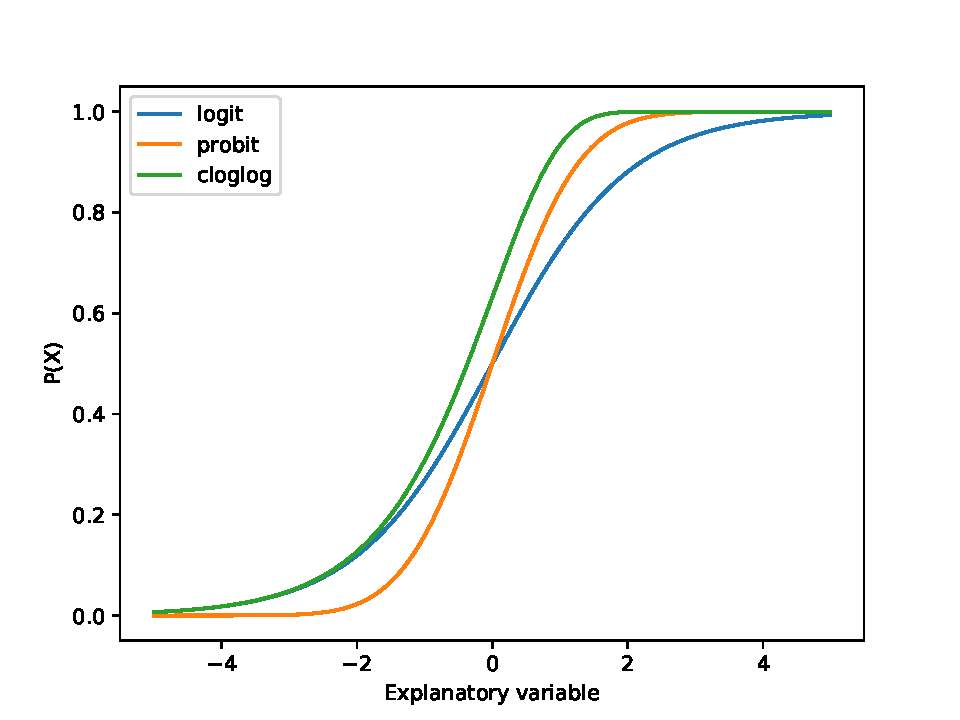
\includegraphics[width=3in]{img/linkfunctions.png}
		\caption{Representation of link functions.}
		\label{fig:linkfunctions}
	\end{figure}
	
	Every convolutional layer is followed by an ELU activation layer~\cite{clevert2015fast} and a batch normalization~\cite{ioffe2015batch}. At the output, a Proportional Odds Model is used with different link functions~\cite{agresti2010analysis}. The logit link function is commonly used within POM. In this paper, we are comparing other link functions like probit or complementary log-log with the logit link. These three types of links are explained below and represented in Figure \ref{fig:linkfunctions}. They all follow the same form $P(y \prec \mathcal{C}_q) = \Phi(b_q-\mathbf{w^Tx})$ for a continuous cdf~$\Phi$.
	
	\begin{itemize}
		\item \textit{Logit}. Logit link function is the most widely used function for Proportional Odds Models. The logit link is shown in \ref{eq:logit} and \ref{eq:logit2}.
		\begin{equation}
		\begin{aligned}
		logit[P(y \preceq \mathcal{C}_q)] = log\frac{P(y \preceq \mathcal{C}_q)}{1 - P(y \preceq \mathcal{C}_q)}=& \\ = b_q - \mathbf{w^Tx}, \quad q = 1, ..., Q-1
		\end{aligned}
		\label{eq:logit}
		\end{equation}
		
		or the equivalent expression
		
		\begin{equation}
		P(y \preceq \mathcal{C}_q) = \frac{1}{1 + e^{-(b-\mathbf{w^Tx})}}
		\label{eq:logit2}
		\end{equation}
		\item \textit{Probit}. Probit link function is the inverse of the standard normal cummulative distribution function (cdf) $\Phi$. Its expression is shown in \ref{eq:probit} and \ref{eq:probit2}.	
		\begin{equation}
		\begin{aligned}
		&\Phi^{-1}[P(y \preceq \mathcal{C}_q)] = b_q - \mathbf{w^Tx}, &q = 1, ..., Q-1\\
		&P(y \preceq \mathcal{C}_q) = \Phi(b_q - \mathbf{w^Tx}), &q = 1, ..., Q-1		
		\end{aligned}
		\label{eq:probit}
		\end{equation}
		
		or
		
		\begin{equation}
		P(y \preceq \mathcal{C}_q) = \int_{-\infty}^{b_q - \mathbf{w^Tx}} \frac{1}{\sqrt{2\pi}} e^{-\frac{1}{2}x^2} dx
		\label{eq:probit2}
		\end{equation}
		
		\item \textit{Complementary log-log}. Like the logit and the probit transformation, the complementary log-log transformation takes a response that is restricted to the (0,1) interval and converts it into something in $(-\infty, +\infty)$ interval. Complementary log-log expression is shown in \ref{eq:cloglog} and \ref{eq:cloglog2}.
		\begin{equation}
		\begin{aligned}
		log[-log[1 - P(y \preceq \mathcal{C}_q)]] =&\\
		= b_q - \mathbf{w^Tx}, \quad q = 1, ..., Q-1&
		\end{aligned}
		\label{eq:cloglog}
		\end{equation}
		
		or
		
		\begin{equation}
		P(y \preceq \mathcal{C}_q) = 1 - e^{-e^{b_q - \mathbf{w^Tx}}}, \quad q = 1, ..., Q-1
		\label{eq:cloglog2}
		\end{equation}
	\end{itemize}
	
	Logit and probit links are symmetric, that is
	
	\begin{equation}
	link[P(y \preceq \mathcal{C}_q)] = -link[1 - P(y \preceq \mathcal{C}_q)]
	\end{equation}
	
	This means that the response curve for $P(y \preceq \mathcal{C}_q)$ has a symmetric appearance about the point $P(y \preceq \mathcal{C}_q) = 0.5$, and so $P(y \preceq \mathcal{C}_q)$ has the same rate for approaching 0 than for approaching 1. This symmetric property can be demonstrated as follows:
	
	\begin{enumerate}
		\item If we define $P(y \preceq \mathcal{C}_q) \equiv p$, we have
			\begin{equation}
			\begin{aligned}
			link(p) = logit(p) &= log\left(\frac{p}{1-p}\right) =\\
			&= log(p) - log(1-p)
			\end{aligned}
			\end{equation}
			
			while
			
			\begin{equation}
			\begin{aligned}
			-link(1 - p) &= -logit(1 - p) =\\
			=- log\left(\frac{1- p}{p}\right) &= - log(1 - p) + log(p)
			\end{aligned}
			\end{equation}
			
			The symmetry has been proven for logit link.
			
		\item If we define 
		
		\begin{equation}
		\begin{aligned}
		p \equiv P(y \preceq \mathcal{C}_q) &= \Phi(b_q - \mathbf{w^Tx}) =\\
		&= \int_{-\infty}^{b_q - \mathbf{w^Tx}} \frac{1}{\sqrt{2\pi}} e^{-\frac{1}{2}x^2} dx
		\end{aligned}
		\end{equation}
		
		then
		
		\begin{equation}
		probit(p) = \Phi^{-1}(p) = b_q - \mathbf{w^Tx}
		\end{equation}
		
		and
		
		\begin{equation}
		-probit(1-p) = \Phi^{-1}(1-p) = -b_q + \mathbf{w^Tx}
		\end{equation}
		
		where
		
		\begin{equation}
		1 - p = \int_{-\infty}^{-b_q + \mathbf{w^Tx}} \frac{1}{\sqrt{2\pi}} e^{-\frac{1}{2}x^2} dx
		\end{equation}
		
		and
		
		\begin{equation}
		p = 1 - \int_{-\infty}^{-b_q + \mathbf{w^Tx}} \frac{1}{\sqrt{2\pi}} e^{-\frac{1}{2}x^2} dx
		\end{equation}

		the symmetric property for the probit function has been proven.
	\end{enumerate}
	
	
	Unlike logit and probit, the complementary log-log model is asymmetrical. It is frequently used when the probability of an event is very small or very large. When the given data is not symmetric in the $[0,1]$ interval and increase slowly at small to moderate value but increases sharply near 1, the logit and probit models are inappropriate. However, in this situation, the complementary log-log model might give a satisfying answer.
	
	\subsection{Procedure}
	The model is optimized using a batch based first-order optimization algorithm called Adam~\cite{kingma2014adam}. We study different initial learning rates in order to find the optimal one for each problem. We apply an exponential decay across training epochs to the initial learning rate.
	
	Both datasets have been artificially equalised using data augmentation techniques~\cite{van2001art, krizhevsky2012imagenet} based on image cropping and zooming, horizontal and vertical flipping, brightness adjustment and random rotations. In the case of Diabetic Retinopathy Detection, the epoch size has been fixed to $100000$ images per epoch. For the Adience dataset, epoch size is the number of images in the training set.
	
	The model is evaluated with Quadratic Weighted Kappa metric (QWK)~\cite{ben2008comparison}. This evaluation measure gives a higher weight to the errors that are further from the correct class. Quadratic weighted kappa loss is considered as loss function for the optimizer as it gives better performance for ordinal classification problems.
	
	Experiments were run with the standard cross-entropy loss and the softmax function too in order to prove the performance improvement of the QWK loss and the Proportional Odds Model. The results of these experiments are analysed in Section \ref{app:NominalComparison}.
	
	\subsection{Factors}
	Three different factors have been considered: learning rate, batch size and link function for the final output layer.
	
	\begin{itemize}
		\item \textit{Learning rate}. Learning rate is one of the most critical hyper-parameters to tune for training deep neural networks. Optimal learning rate can vary depending on the dataset and the CNN architecture. Previous works have presented some techniques that adjust this parameter in order to achieve better performance~\cite{smith2017cyclical, senior2013empirical}. Within this work, we have considered three different values for this parameter: $10^{-2}$, $10^{-3}$ and $10^{-4}$.
		\item \textit{Batch size}. Batch size is also an important parameter as it controls the number of weight updates that are made on every epoch. It can affect the training time and the model performance. In this paper, we have tried three separate batch sizes: $5$, $10$ and $15$.
		\item \textit{Link function}. Different link functions have been used for the POM at the last layer output: logit, probit and complementary log-log.
	\end{itemize}
	
	\section{Results}
	\label{sect:results}
	In this section, we present the results of the experiments. For each dataset, we show a table with the detailed experiments done training the model with each combination of parameters. Every parameter combination has been run five times. These tables show the average quadratic weighted kappa across these five executions for validation and test values.
	
	\subsection{Diabetic Retinopathy}
	\label{sect:dr}
	Detailed results for the Diabetic Retinopathy dataset are presented in Table \ref{table:DRresults}.
	
	\begin{table}[!t]
		\caption{Diabetic Retinopathy results. BS stands for Batch Size, LR for Learning Rate and LF for link function.}
		\label{table:DRresults}
		\footnotesize
		\centering
		\begin{tabular}{ccc|cc}
			BS & LR & LF & $\kappa_{val}$ & $\kappa_{test}$\\\hline
			$5$ & $10^{-2}$ & Logit & $0.44888$ & $0.41630$\\
			& & Probit & $0.46724$ & $0.45972$\\
			& & c log-log & $0.42854$ & $0.41448$\\
			& $10^{-3}$ & Logit & $0.56496$ & $0.55356$\\
			& & Probit & $0.57084$ & $0.56392$\\
			& & c log-log & $0.54796$ & $0.53436$\\
			& $10^{-4}$ & Logit & $0.52884$ & $0.52032$\\
			& & Probit & $0.53802$ & $0.52302$\\
			& & c log-log & $0.53824$ & $0.51974$\\
			$10$ & $10^{-2}$ & Logit & $0.54970$ & $0.53142$\\
			& & Probit & $0.52124$ & $0.50806$\\
			& & c log-log & $0.42760$ & $0.42270$\\
			& $10^{-3}$ & Logit & $0.58036$ & $0.57686$\\
			& & Probit & $0.56536$ & $0.55810$\\
			& & c log-log & $\textbf{0.58830}$ & $\textbf{0.58150}$\\
			& $10^{-4}$ & Logit & $0.53158$ & $0.53850$\\
			& & Probit & $0.54560$ & $0.54082$\\
			& & c log-log & $0.53928$ & $0.53742$\\
			$15$ & $10^{-2}$ & Logit & $0.55828$ & $0.55076$\\
			& & Probit & $0.54112$ & $0.53430$\\
			& & c log-log & $0.56676$ & $0.56428$\\
			& $10^{-3}$ & Logit & $0.55748$ & $0.55106$\\
			& & Probit & $0.58182$ & $0.57894$\\
			& & c log-log & $0.56340$ & $0.55938$\\
			& $10^{-4}$ & Logit & $0.54686$ & $0.54342$\\
			& & Probit & $0.53258$ & $0.53278$\\
			& & c log-log & $0.53900$ & $0.53828$
		\end{tabular}
	\end{table}
	
	The best mean QWK value was obtained with the complementary log-log link function using a batch size of 10 and a learning rate of $10^{-3}$.
	
	\subsection{Adience}
	\label{sect:adience}
	Results for the experiments made with the Adience dataset are shown in Table \ref{table:Adienceresults}.
	
	\begin{table}[!t]
		\caption{Adience results. BS stands for Batch Size, LR for Learning Rate and LF for link function.}
		\label{table:Adienceresults}
		\footnotesize
		\centering
		\begin{tabular}{ccc|cc}
			BS & LR & LF & $\kappa_{val}$ & $\kappa_{test}$\\\hline
			$5$ & $10^{-2}$ & Logit & $0.72072$ & $0.68408$\\
			& & Probit & $0.77608$ & $0.72574$\\
			& & c log-log & $0.75430$ & $0.70742$\\
			& $10^{-3}$ & Logit & $0.71460$ & $0.67868$\\
			& & Probit & $0.81906$ & $0.77154$\\
			& & c log-log & $0.57196$ & $0.55608$\\
			& $10^{-4}$ & Logit & $0.54432$ & $0.51934$\\
			& & Probit & $0.54360$ & $0.52422$\\
			& & c log-log & $0.54802$ & $0.52484$\\
			$10$ & $10^{-2}$ & Logit & $0.78872$ & $0.72994$\\
			& & Probit & $0.79332$ & $0.74750$\\
			& & c log-log & $0.78004$ & $0.73260$\\
			& $10^{-3}$ & Logit & $0.49686$ & $0.47112$\\
			& & Probit & $0.59778$ & $0.58476$\\
			& & c log-log & $0.52016$ & $0.49968$\\
			& $10^{-4}$ & Logit & $0.60972$ & $0.56814$\\
			& & Probit & $0.54638$ & $0.52632$\\
			& & c log-log & $0.75428$ & $0.52094$\\
			$15$ & $10^{-2}$ & Logit & $0.79104$ & $0.74388$\\
			& & Probit & $\textbf{0.84254}$ & $\textbf{0.78666}$\\
			& & c log-log & $0.78802$ & $0.74624$\\
			& $10^{-3}$ & Logit & $0.56946$ & $0.52978$\\
			& & Probit & $0.70262$ & $0.65416$\\
			& & c log-log & $0.49242$ & $0.47320$\\
			& $10^{-4}$ & Logit & $0.55202$ & $0.52484$\\
			& & Probit & $0.54288$ & $0.51740$\\
			& & c log-log & $0.53826$ & $0.52542$
		\end{tabular}
		
	\end{table}
	
	The best mean QWK value was obtained with the probit link function using a batch size of 15 and a learning rate of $10^{-2}$.
	
	\subsection{Statistical analysis}
	\label{sect:statisticalanalysis}
	In this subsection, a statistical analysis will be performed in order to obtain conclusions from the results presented in this section.
	
	The significance and relative importance of the parameters concerning the results obtained, as well as suitable values for each, were obtained using the ANalysis Of the VAriance (ANOVA) test.
	
	The ANOVA test~\cite{miller1997beyond} is one of the most widely used statistical techniques. ANOVA is essentially a method of analysing the variance to which a response is subject into its various components, corresponding to the sources of variation which can be identified.
	
	ANOVA, in this case, examines the effects of three quantitative variables (termed factors) on one quantitative response. Considered factors are the link function, which can be logit, probit and complementary log-log, the learning rate for the Adam optimization algorithm ($10^{-2}$, $10^{-3}$ and $10^{-4}$) and the batch size (5, 10 and 15).
	
	Following the setup of the previous study, we performed an ANOVA III analysis and multiple comparison tests. We assume that five executions are enough to do the statistical tests because of the computational time limitations.
	
	The test shows that there is no batch size whose results are significatively better than the results of all other batch sizes. This does not mean that these differences could not exist for specific numbers of samples per batch. So, in order to determine for each type of function whether a batch size is better than the others, we have performed an ANOVA I analysis - where the only factor is the batch size - and multiple comparison tests.
	
	We denote by $QWK_{i,j,k,l}(i=1, ..., 3; j = 1, ..., 3; k = 1, ..., 3)$ the value observed when the first factor is at the i-th level, the second at the j-th level and the third at k-th level. We assume that the three factors do not act independently and therefore there exists an interaction between each pair of them and between the three factors. In this case, the observations fit \ref{eq:anova3}.
	
	\begin{equation}
	\begin{aligned}
	\footnotesize
	QWK_{i,j,k,l} = & \mu + L_i + P_j + B_k + LP_{i,j} + LB_{i,k} \\& + PB_{j,k} + LPB_{i,j,k} + \epsilon_{i,j,k,l}
	\label{eq:anova3}
	\end{aligned}
	\end{equation}
	
	where $\mu$ is the fixed effect that is common to all the populations; $L_i$ is the effect associated with the \textit{i-th} level of the link factor (logit, probit, complementary log-log); $P_j$ is the effect associated with the \textit{j-th} level of the parameter factor ($10^{-4}$, $10^{-3}$, $10^{-2}$) and $B_k$ is the effect associated with the \textit{k-th} level of the batch size factor (5, 10, 15). The term $LP_{i,j}$ denotes the joint effect of the presence of level $i$ of the first factor and level $j$ of the second one; this, therefore, is denominated the interaction term between $L$ and $P$ factors. The same interaction effect is appreciated on $LB_{i,k}$, $PB_{j,k}$ and $LPB_{i,j,k}$. The term $\epsilon_{i,j,k,l}$ is the influence on the result of everything that could not be assigned or of random factors. $W_{i,j,k,l}$ is the quadratic weighted kappa measure, the response variable used to perform the statistical analysis.
	
	We consider some hypotheses testing where the null hypothesis is proposed that each term of the above equation is independent of the levels involved. The hypotheses for the levels of the L factor are
	\[
	H_0 \equiv L_1 = L_2 = L_3
	\]
	\[
	H_1 \equiv \text{ some } L_i \text{ is different}
	\]
	
	The same hypotheses are made for the other factors. In this way, we test in the null hypothesis that all of the population means are equal against an alternative hypothesis that there is at least one mean that is not equal to the others.
	
	The hypothesis associated with the interaction between L and P is
	\[
	H_0 \equiv LP_{i,j} = 0 \quad \forall i,j
	\]
	\[
	H_1 \equiv \exists LP_{i,j} \ne 0
	\]
	
	Similar hypotheses can be assumed for the interaction between the other factors.
	
	The analysis of variance table containing the sum of squares, degrees of freedom, mean square, test statistics and significance level represent the initial study in a compact form, where non-significative factors and interactions have been removed ($\text{p-value} > 0.05$). These factors and interactions take part of the error component now.
	
	\begin{table}[!t]
		\caption{ANOVA III for the analysis of the main factors in the design of a Convolutional Ordinal Neural Network for the Retinopathy dataset.}
		\label{table:ANOVARetinopathy}
		\centering
		\small
		\begin{tabular}{l|ccccc}
			\multicolumn{6}{c}{Response variable QWK}\\\hline
			Source & S.S. & D.F. & M.S. & F-ratio & Sig.\\\hline
			Model & $37.860$ & $9$ & $4.207$ & $1562.840$ & $0.000$\\
			$L$ factor & $0.057$ & $2$ & $0.029$ & $10.646$ & $0.000$\\
			$P$ factor & $0.121$ & $2$ & $0.060$ & $22.468$ & $0.000$\\
			$LP$ factors & $0.057$ & $4$ & $0.014$ & $5.261$ & $0.001$\\
			Error & $0.339$ & $126$ & $0.003$ & & \\
			Total & $38.199$ & $135$ & & & 
		\end{tabular}
	\end{table}
	
	The results of the ANOVA III test for the Diabetic Retinopathy dataset are resumed in Table \ref{table:ANOVARetinopathy}. There are significative differences in the means of QWK depending on the link function and also depending on the learning rate for $\alpha=0.05$. Moreover, an interaction between the link function and the learning rate can be recognised ($\text{p-value} = 0.001$).
	
	As Table \ref{table:ANOVARetinopathy} showed that there exist significative differences between the means, we are now analysing those differences. A post-hoc multiple comparison test has been performed on the mean QWK obtained. An HSD Tukey's test was made under the null hypothesis that the variance of the error of the dependent variable is the same between groups. The best link function is the complementary log-log, though it doesn't have significative differences with the probit function ($\alpha=0.05$). There are differences between the complementary log-log and the probit function concerning the logit function.
	
	The results have been obtained following a similar methodology with the different values of the learning parameter including the HSD Tukey's test and the learning parameter ranking. Significative differences can be observed in the mean values for $\eta = 10^{-3}$ with respect to the other values of the parameter ($\alpha=0.05$). Also, there are differences for $\eta = 10^{-4}$ concerning $\eta = 10^{-2}$.
	
	\begin{table}[!t]
		\caption{ANOVA III for the analysis of the main factors in the design of a Convolutional Ordinal Neural Network for the Adience dataset.}
		\label{table:ANOVAAdience}
		\centering
		\small
		\begin{tabular}{l|ccccc}
			\multicolumn{6}{c}{Response variable QWK}\\\hline
			Source & S.S. & D.F. & M.S. & F-ratio & Sig.\\\hline
			Model & $52.328$ & $15$ & $3.489$ & $1426.170$ & $0.000$\\
			$L$ factor & $0.027$ & $2$ & $0.014$ & $5.582$ & $0.005$\\
			$P$ factor & $1.031$ & $2$ & $0.516$ & $210.809$ & $0.000$\\
			$B$ factor & $0.089$ & $2$ & $0.045$ & $18.253$ & $0.000$\\
			$LP$ factors & $0.183$ & $4$ & $0.046$ & $18.695$ & $0.000$\\
			$PB$ factors & $0.124$ & $4$ & $0.031$ & $12.695$ & $0.000$\\
			Error & $0.294$ & $120$ & $0.002$ & & \\
			Total & $52.622$ & $135$ & $3.489$ & & 
		\end{tabular}
	\end{table}
	
	The results of the ANOVA III test for the Adience dataset are shown in Table \ref{table:ANOVAAdience}. The interactions where there are not significative differences in QWK means have been omitted. First, the factor associated with the link function is analysed. The differences between the means are significative ($\text{p-value} = 0.005$). Secondly, there are significative differences concerning the learning rate factor too ($\text{p-value} = 0.000$). Also, there are differences for the means of QWK for the batch size factor. Significative interactions exist between two pairs of factors: link function and learning rate, and learning rate and batch size ($\text{p-value = 0.000}$ for both cases).
	
	A post-hoc multiple comparison test has been performed on the average QWK obtained for this dataset too. Under the null hypothesis that the variance of the error of the dependent variable is the same between groups, an HSD Tukey's test has been done. The results showed that the best link function is the logit one, in this case, with $0.60553$ as mean QWK value. However, there are not significative differences between this function and the complementary log-log ($\text{p-value}=0.110$). It has differences with the probit function though ($\text{p-value} = 0.003$). The complementary log-log link reported the best results after the logit function, having a mean QWK of $0.58738$. However, it doesn't show significative differences with the probit function.
	The results have been obtained following a similar methodology with the different values of the learning parameter including the HSD Tukey's test and the learning parameter ranking. The test reported significative differences between $\eta=10^{-2}$ (mean value $0.73378$) and the rest of values of this parameter ($\alpha=0.005$), being this one the best value for this factor. The best value after $10^{-2}$ is $10^{-3}$, which have a mean QWK value of $0.57989$. Lastly, the best value for the batch size parameter is $5$ (mean value $0.63243$) as it has significative differences with the rest of values. The second best value is $15$ (mean $0.61129$), but it has no significative differences with $10$ ($\text{p-value}= 0.194$).
	
	To sum up, the results showed that the best parameter configuration depends on the problem that is being solved. None of the optimal parameters is the same for Retinopathy and Adience datasets. These results highlight the importance of adjusting the hyper-parameters for each problem that is treated instead of trying to find an optimal configuration for all the datasets.
	
	\subsection{Statistical comparison between nominal and ordinal methods}
	\label{app:NominalComparison}
	
	The same experiments described in Section \ref{sect:experiments} were repeated using the cross-entropy instead of the QWK as loss function for the optimizer and the softmax function instead of the Proportional Odds Model for the output of the network. The evaluation metric remains the same in order to be able to compare. The results for both datasets are shown in Table \ref{table:NominalResults}. There are some parameter configurations where the training process gets stagnated and a very low QWK is obtained. As we saw in Sections \ref{sect:dr} and \ref{sect:adience}, this problem is not present when using the ordinal method.
	
	\begin{table}[!t]
		\caption{Nominal method results. BS stands for Batch Size and LR for Learning Rate.}
		\label{table:NominalResults}
		\footnotesize
		\centering
		\begin{tabular}{lcc|cc}
			Dataset & BS & LR & $\kappa_{val}$ & $\kappa_{test}$\\\hline
			Retinopathy & $5$ & $10^{-2}$ & $0.2210$ & $0.2050$\\
			 & & $10^{-3}$ & $0.2807$ & $0.2654$\\
			 & & $10^{-4}$ & $0.4580$ & $0.4449$\\
			
			 & $10$ & $10^{-2}$ & $0.2972$ & $0.2997$\\
			 &  & $10^{-3}$ & $0.3972$ & $0.3989$\\
			 &  & $10^{-4}$ & $\textbf{0.4972}$ & $\textbf{0.4967}$\\
			
			 & $15$ & $10^{-2}$ & $0.3692$ & $0.3676$\\
			 & & $10^{-3}$ & $0.4107$ & $0.4162$\\
			 & & $10^{-4}$ & $0.4929$ & $0.4859$\\
			\hline
			Adience & $5$ & $10^{-2}$ & $0.0605$ & $0.0769$\\
			 & & $10^{-3}$ & $0.7994$ & $0.7313$\\
			 & & $10^{-4}$ & $0.8009$ & $0.7383$\\
			
			 & $10$ & $10^{-2}$ & $0.0559$ & $0.0576$\\
			 & & $10^{-3}$ & $0.8239$ & $0.7436$\\
			 & & $10^{-4}$ & $0.7938$ & $0.7218$\\
			
			 & $15$ & $10^{-2}$ & $0.0593$ & $0.0713$\\
			 & & $10^{-3}$ & $\textbf{0.8309}$ & $\textbf{0.7575}$\\
			 & & $10^{-4}$ & $0.7867$ & $0.7129$\\
		\end{tabular}
	\end{table}
	
	As we did in Section \ref{sect:statisticalanalysis}, we must analyse the effect of the batch size (with values 5, 10 and 15) and the learning rate ($10^{-2}$, $10^{-3}$ and $10^{-4}$) factors have over the QWK metric. So, we make an ANOVA II analysis for each dataset.
	
	In the Diabetic Retinopathy dataset, there are significative differences between the mean values of QWK depending on the batch size and the initial value of the learning rate. Also, no significative interaction was detected between these factors.
	
	After that, a post-hoc Tukey's test shows that the best value for the batch size factor is 15 followed by 10. However, there are no significative differences between them, but there are differences with size 5. Also, the best value for the learning rate is $10^{-4}$ and there are significative differences with the rest of values.
	
	A similar study was made for the Adience dataset. There are not significative differences for the mean value of QWK w.r.t. the batch size factor. Also, there are no interactions between the batch size and the learning rate. The best results were obtained with $10^{-3}$ for the learning rate followed by $10^{-4}$, without significative differences between them.
	
	The conclusions obtained from the results are exposed below:
	\begin{itemize}
		\item There are no interactions between both factors.
		\item Batch sizes 10 and 15 obtained the best results.
		\item Learning rate $10^{-4}$ is the best choice for both datasets as it the best for Diabetic Retinopathy, with significative differences, and it is the second for Adience, without significative differences with the best. 
	\end{itemize}
	

	Finally, a comparison of the best QWK for each dataset for ordinal and nominal cases is shown in Table \ref{table:ComparisonNomOrd}. Also, it is compared with previous works. The proposed ordinal model outperforms all the other alternatives. The performance increase of POM over softmax reaches $17.07\%$ for Diabetic Retinopathy and $3.85\%$ for Adience dataset. The enhancement of the ordinal method for Retinopathy dataset is more notable than the rise for Adience dataset. It seems that the method proposed in this work offers a more significant improvement as the given problem complexity increases.
	
	\begin{table}[!t]
		\caption{Comparison between the best QWK results of nominal, ordinal and previous works.}
		\label{table:ComparisonNomOrd}
		\footnotesize
		\centering
		\begin{tabular}{lccc|cc}
			\multicolumn{6}{c}{Diabetic Retinopathy}\\
			\hline
			Method & BS & LR & LF & $\kappa_{val}$ & $\kappa_{test}$\\\hline
			Ord. proposed & 10 & $10^{-3}$ & c log-log & $0.58830$ & $0.58150$\\
			Nom. proposed & 10 & $10^{-4}$ & softmax & $0.49720$ & $0.49670$\\
			Best from \cite{de2018weighted} & 20 & $10^{-4}$ & softmax & $0.53700$ & -\\
			Best from \cite{nebot2016diabetic} & - & - & softmax & - & $0.55500$\\
			\hline\hline
			\multicolumn{6}{c}{Adience}\\
			\hline
			Ord. proposed & 15 & $10^{-2}$ & probit & $0.84254$ & $0.78666$\\
			Nom. proposed & 15 & $10^{-3}$ & softmax & $0.83090$ & $0.75750$\\
		\end{tabular}
	\end{table}
	
	\section{Conclusions}
	\label{sect:conclusions}
	In this section, the conclusions obtained from this work are exposed. The first thing that we have noticed is that the optimal values for the different parameters considered are problem-dependant. 
	
	The complementary log-log function has the best average performance across both datasets. It offers the best results in Diabetic Retinopathy dataset and the second best result in Adience dataset. These results provide an opportunity for exploring new generalised link functions.
	
	The best value for the learning rate parameter for  Diabetic Retinopathy dataset is $\eta = 10^{-3}$ while this value is the second best option for Adience dataset. It can be considered a good value for this parameter when training the model with new datasets.
	
	Both datasets have obtained the best performance with batch size 10.
	
	Also, the statistical tests reported that there are interactions between some parameters like the link function and the learning rate, for Diabetic Retinopathy, or those factors in addition to learning rate and batch size, for Adience dataset.
	
	The proposed POM has improved the performance of the deep network regarding quadratic weighted kappa compared to the model that uses the softmax function. This enhancement is more notable for the Diabetic Retinopathy dataset. Also, it reduces the chance that the model gets stuck when training with some parameter configurations. So, the most significant improvements of these link functions are the QWK performance increase, the reduction of the number of parameters configurations that should be tried to find the best one and the prevention of the over-fitting and the stagnation.
	
	
	% if have a single appendix:
	%\appendix[Proof of the Zonklar Equations]
	% or
	%\appendix  % for no appendix heading
	% do not use \section anymore after \appendix, only \section*
	% is possibly needed
	
	% use appendices with more than one appendix
	% then use \section to start each appendix
	% you must declare a \section before using any
	% \subsection or using \label (\appendices by itself
	% starts a section numbered zero.)
	%
	
	

	
	
	% Can use something like this to put references on a page
	% by themselves when using endfloat and the captionsoff option.
	\ifCLASSOPTIONcaptionsoff
	\newpage
	\fi
	
	
	
	% trigger a \newpage just before the given reference
	% number - used to balance the columns on the last page
	% adjust value as needed - may need to be readjusted if
	% the document is modified later
	%\IEEEtriggeratref{8}
	% The "triggered" command can be changed if desired:
	%\IEEEtriggercmd{\enlargethispage{-5in}}
	
	% references section
	
	% can use a bibliography generated by BibTeX as a .bbl file
	% BibTeX documentation can be easily obtained at:
	% http://mirror.ctan.org/biblio/bibtex/contrib/doc/
	% The IEEEtran BibTeX style support page is at:
	% http://www.michaelshell.org/tex/ieeetran/bibtex/
	%\bibliographystyle{IEEEtran}
	% argument is your BibTeX string definitions and bibliography database(s)
	%\bibliography{IEEEabrv,../bib/paper}
	%
	% <OR> manually copy in the resultant .bbl file
	% set second argument of \begin to the number of references
	% (used to reserve space for the reference number labels box)

	\printbibliography
		

	
	
	
	% You can push biographies down or up by placing
	% a \vfill before or after them. The appropriate
	% use of \vfill depends on what kind of text is
	% on the last page and whether or not the columns
	% are being equalized.
	
	%\vfill
	
	% Can be used to pull up biographies so that the bottom of the last one
	% is flush with the other column.
	%\enlargethispage{-5in}
	
	
	
	% that's all folks
\end{document}


